

\chapter{Introduction}

Performing a movement is a complicated process that involves many physiological entities working in high coherence. It involves bones, tendons, nerves, and many other working in perfect harmony. Even the simplest movements are rarely performed using just one muscle. Everything we do involves high muscular coordination and constant and precise regulation. While standing, muscles of legs and trunk are constantly simultaneously co-contracting, maintaining balance.  
Muscle is a body tissue capable of transforming chemical energy to force. There are several muscle types: smooth, building internal organs, cardiac, building the heart, and skeletal. Only skeletal muscles can be controlled voluntarily and are used in locomotion. They are usually connected to bones with tendons (collagen fibers), as shown in figure \ref{fig:muscle}.
\begin{figure}[ht]
\centering
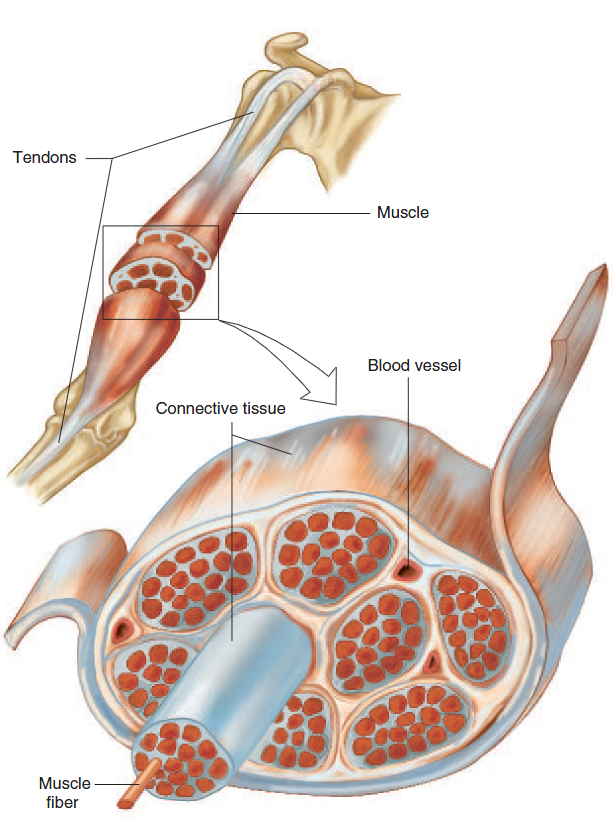
\includegraphics[width=0.5\textwidth]{Images/introduction/muscle.png}
\caption{Organization of skeletal muscle with attachment to the bone. Retrieved from \citep{Widmaier2014}}
\label{fig:muscle}
\end{figure}

The neurons controlling the movement are organized in hierarchical fashion \citep{Widmaier2014}. In the highest level of hierarchy, the movement is conceived. Here the complex plan of intention is made. Very little is known about the exact location of neurons responsible for this task. Higher centers then transmit this command to the middle level structures, where the task is elaborated. Simultaneously, this middle level neurons receive the information from the receptors in muscles, skin, tendons, and join, but also from the visual system. Planning of the movement that is about to be performed is performed with respect to the space this movement will occupy, and detailed control signals for each muscle involved in the movement are generated. Centers involved in this tasks are located in cerebral cortex, cerebellum, subcortical nuclei, and brainstem. The information is then transmitted to the lowest level of the motor hierarchy: spinal cord and brainstem. Here the information is transmitted over motor neurons to the muscles. The selection of motor neurons involved in the task and timing is performed at this level. Organization and locations of the neural system for motor control can be seen in figure \ref{fig:brain_centers}. 
\begin{figure*}[t!]
    \centering
    \begin{subfigure}[t]{0.95\textwidth}
        \centering
        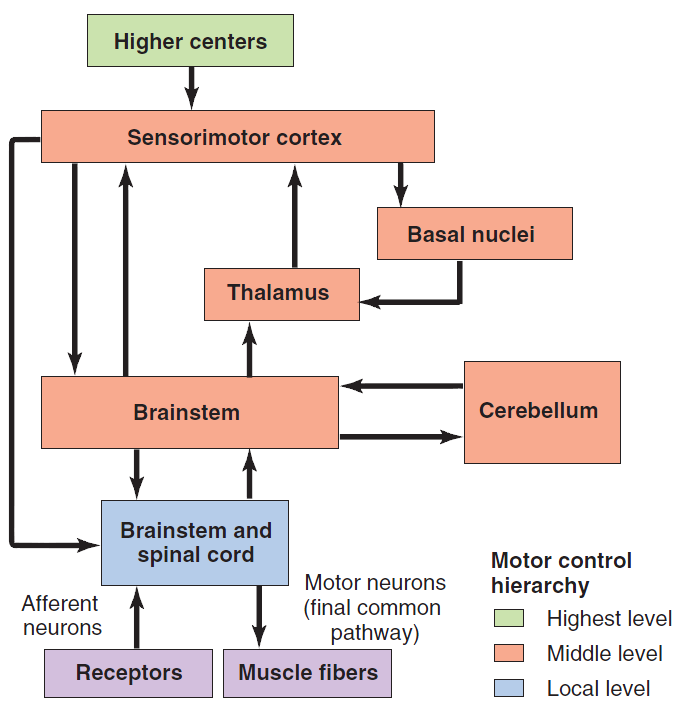
\includegraphics[height=3in]{Images/introduction/control.png}
        \caption{}
    \end{subfigure}%
    
    \begin{subfigure}[t]{0.95\textwidth}
        \centering
        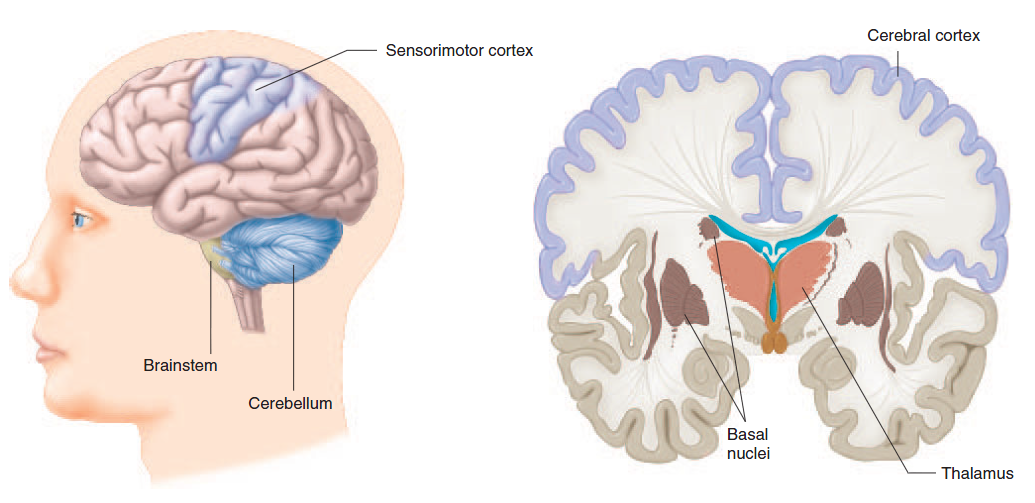
\includegraphics[height=3in]{Images/introduction/control2.png}
        \caption{}
    \end{subfigure}
    \caption{Figure describes \textbf{a)} hierarchical organization of neural system for motor control and \textbf{b)} side view and cross section of the brain showing motor control centers. Retrieved from \citep{Widmaier2014}}
\label{fig:brain_centers}
\end{figure*}

\section{Muscle physiology}

Elementary building block of a muscle is muscle cell, or muscle fiber - \emph{myocyte}. They are ensheated by \emph{endomysium}, a connective tissue that contains nerves and capillaries. Myocytes are organized in bundles of 10 to 100 fibers, which are called \emph{fascicles}, and they are surrounded by sheath of connective tissue, \emph{perymisium}. Group of fascicles is finally grouped together and enveloped by \emph{epimysium}, forming a muscle.

\emph{Sarcolema} is the cell membrane of myocyte, consisting of a lipid bilayer that contains intracelular liquid, \emph{myoplasma}. In the myoplasma, thin and thick filaments are serially connected, forming \emph{sarcomeres}, which are longitudinally connected in \emph{myofibrils} that extend through entire length of the myocyte. During shortening of muscle fibers, thin and thick filaments of sarcomeres are pulled together by cross-bridges between them. Total shortening of myofibril is summation of shortenings of sarcomeres of which it is composed.

Each motor neuron at the neuromuscular junction innervates several muscle fibers, forming the smallest functional unit called \emph{motor unit}. It was firstly defined by Liddell and Sherrington in 1925 \citep{Liddell1925, Sherrington1925} and is composed of motor neuron with axon and dendrites, and muscle fibers that axon innervates \citep{Duchateau2011}. Since motor neuron with a single action potential usually evokes action potentials simultaneously in all belonging muscle fibers, by observing action potentials of the muscle fibers, information on activity of motor neurons in spinal cord or brain stem can be inferred \citep{Merletti-Farina-book}. Pool of motor neurons that innervates entire muscle generally ranges from ten to thousand, depending on the muscle \citep{Merletti-Farina-book}.

By the characteristics of muscle fiber, there are three main types of muscle fibers:
\begin{description}
\item[Fast twitch, fatigable fibers (FF, or type IIb):] This fiber type have high levels of ATP (source of energy) for anaerobic energy supply, and are dominantly present in pale muscles. They are of glycolytic type and work well in ischemic or low oxygen conditions. Regarding contraction properties, they are characterized by fast twitch, large forces and high nerve conduction velocity, but they get fatigued faster than the other muscle fiber types. 

\item[Fast twitch, fatigue-resistant (FR, or type IIa):] These are oxidative glycolytic fibers, characterized by fast twitch and are resistant to fatigue. They have intermediate conduction velocity. 

\item[Slow twitch, very resistant to fatigue (S, or type I):] They are slow oxidative fibers and do not work well in low oxygen conditions. They generate small forces, have slow twitch and are characterized by lower nerve conduction velocity. This fiber type is very resilient to fatigue because of high oxidative metabolism and energy efficiency. They are present in high percentage in red muscles, such as soleus.
\end{description}

Muscle fibers innervated by the same motor neuron have similar histochemical and contractile characteristics, and can be said that motor unit is composed of the muscle fibers of the same type.

Force that muscle fibers generate depends on firing frequency of the action potentials (rate coding) innervating the neuromuscular junction, and the recruitment strategy by which the motor units are activated, i.e., the number of activated motor units. Firing frequency and the recruitment strategy depend on the speed and force of contraction. Muscle units with low threshold are activated firstly, resulting in low force and high endurance, i.e., resistance to fatigue. If greater force is required, muscle units with higher threshold that are prone to fatigue are activated \citep{Freund1975, Merletti-book}. This was firstly proposed by Henneman et al. in 1965 \citep{Henneman1965}, who state that order of recruitment of motor neurons is based on size principle, that is, neurons with smaller axons are recruited at lower effort levels and with increase in force, larger motoneurons are recruited. Therefore, S type muscle units, which have the smallest motoneurons are recruited first, followed by FR type units, and finally FF units. The recruitment strategy and resistance to fatigue can be seen in figure \ref{fig:fibers}. 

%\begin{figure}[ht]
%\centering
%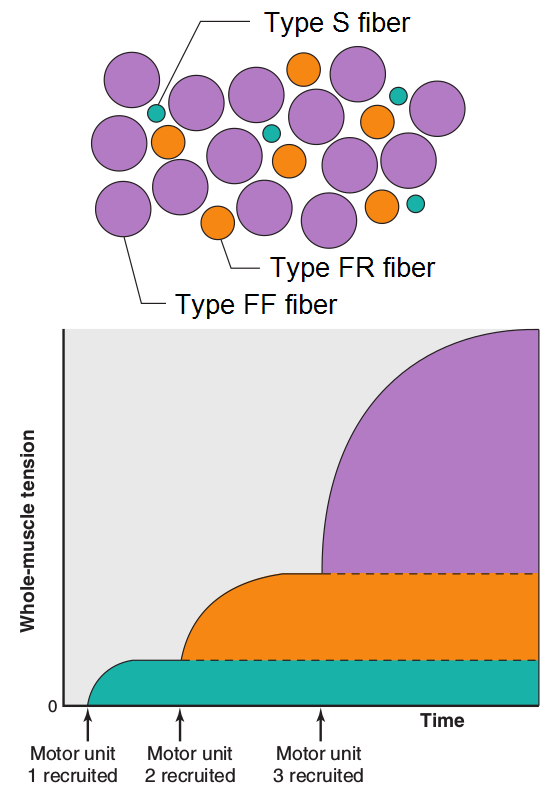
\includegraphics[width=0.5\textwidth]{Images/introduction/fiber_distribution.png}
%\caption{Figure illustrates \textbf{a)} diagram of different muscle fibers in muscle cross section, and \textbf{b)} muscle tension produced by recruitment of different types of muscle fiber. It can be noted that type S fibers are activated first and generate low force level, whereas type FF fibers are activated last and generate high forces . Adopted from Widmaier}
%\label{fig:fiber_distribution}
%\end{figure}
%
%\begin{figure}[ht]
%\centering
%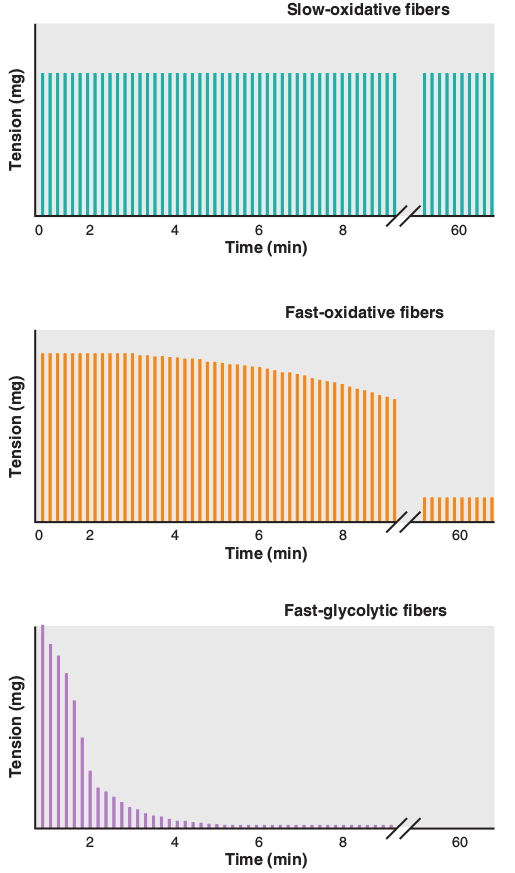
\includegraphics[width=0.5\textwidth]{Images/introduction/fiber_fatigue.png}
%\caption{Figure illustrates the time during which specific muscle fibers can remain tension. Adopted from Widmaier}
%\label{fig:fiber_fatigue}
%\end{figure}

\begin{figure*}[t!]
    \centering
    \begin{subfigure}[t]{0.45\textwidth}
        \centering
        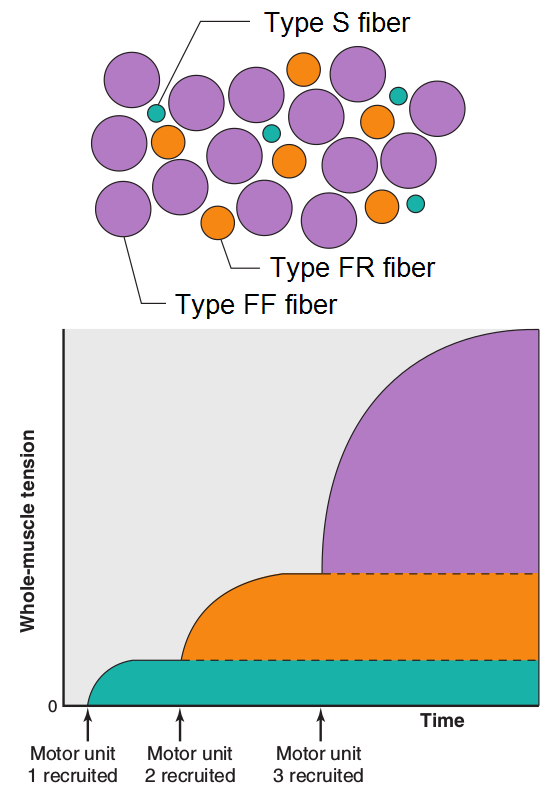
\includegraphics[height=4in]{Images/introduction/fiber_distribution.png}
        \caption{}
    \end{subfigure}%
    ~ 
    \begin{subfigure}[t]{0.45\textwidth}
        \centering
        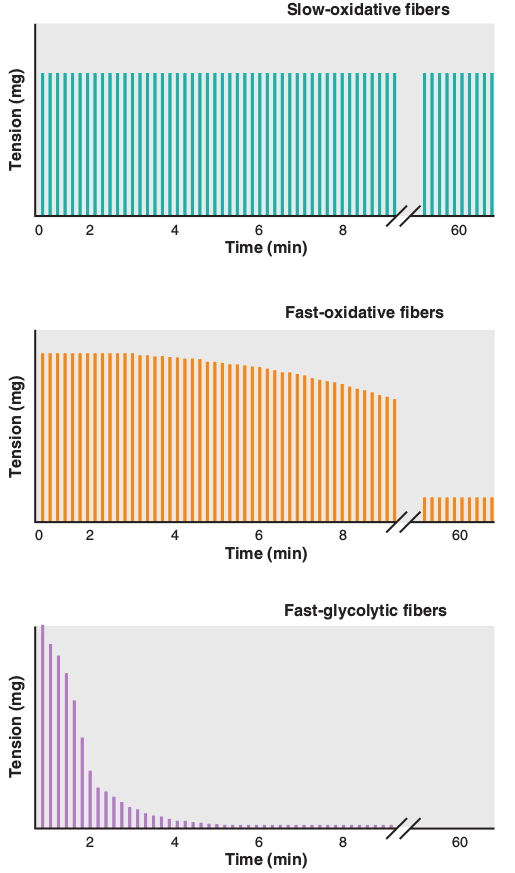
\includegraphics[height=4in]{Images/introduction/fiber_fatigue.png}
        \caption{}
    \end{subfigure}
    \caption{Figure describes characteristics of different types of muscle fibers. In \textbf{a)} is a diagram of different muscle fibers in muscle cross section (top), and muscle tension produced by recruitment of different types of muscle fiber (bottom), whereas in \textbf{b)} is the illustration of the time interval during which specific muscle fibers can remain tension. It can be noted that type S fibers are activated first, generate low force level, and are resistant to fatigue. On the other hand, type FF fibers are activated last, generate high forces, and develop fatigue fastest. Retrieved from \citep{Widmaier2014}}
\label{fig:fibers}
\end{figure*}


\section{Muscle contraction}

Skeletal muscles are activated voluntarily by electro-chemical impulses of motor neurons. The process is described in this chapter in summarized version. For more detailed description, the reader is pointed to medical literature (e.g. {Widmaier2014}).

During the stable state when there are no stimuli, i.e., in the resting state, the interior of the myocyte is at higher electrical potential that the exterior. This difference in potential is usually around 80 mV and it is caused by the higher concentration of positive ions, namely Na+, outside of the sarcolema \citep{Nazmi2016}, as shown in figure \ref{fig:depolarization}.

\begin{figure}[ht]
\centering
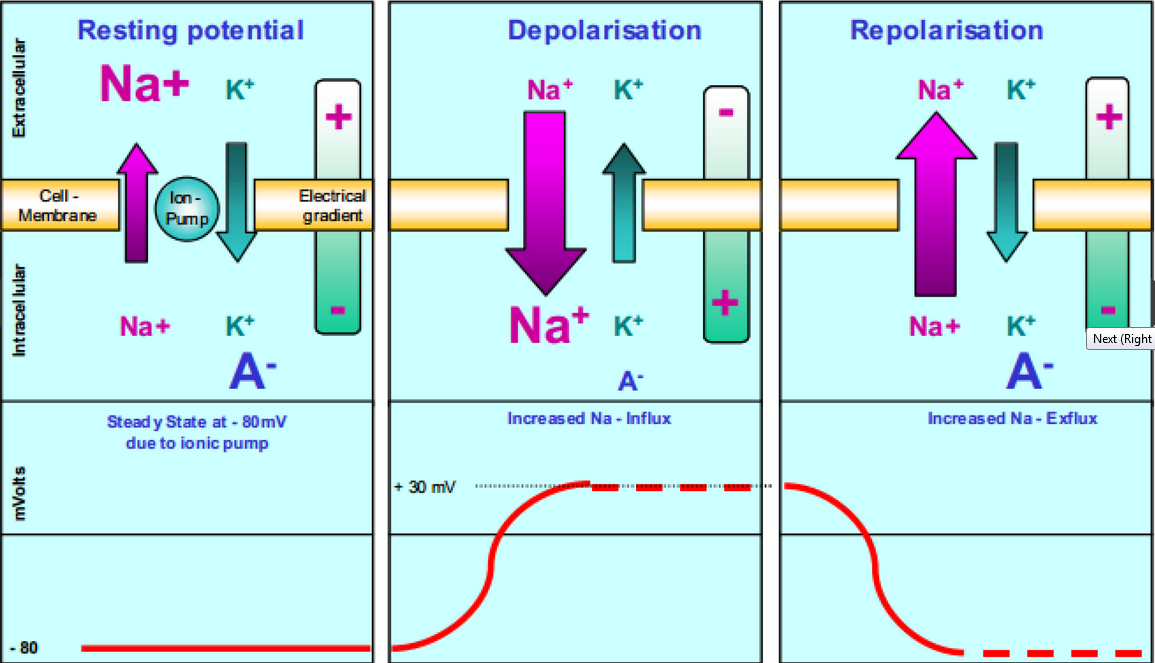
\includegraphics[width=0.95\textwidth]{Images/introduction/Depolarization.png}
\caption{Ilustration of depolarization/repolarization of the muscle fiber. Adopted from \citep{Nazmi2016}.}
\label{fig:depolarization}
\end{figure}

Motor neurons transfer nerve impulses that control the muscle from spinal cord to neuromuscular junction. At the nerve endings, action potentials induce the opening of calcium channels, which enables calcium from extracellular fluid to enter axon terminals and trigger the release of the neurotransmitter \emph{acetylcholine}. Acetylcholine is released to the narrow space between the axon and sarcolema of the myocyte, and causes sodium channels in sarcolema to open and allow the flow of Na+ and K+ ions in both directions. Na+ ions now flow into the myoplasma by diffusion due to higher concentration of Na+ ions outside of the membrane, but because of similar gradient, concentrations of the K+ ions don't change a lot. This process causes depolarization of sarcolema during which the outside potential of the muscle cell is at lower voltage than inside potential by around 30 mV. Depolarization is immediately followed by repolarization, a process during which the electrochemical balance and the resting potential of the cell are restored. It is achieved by flushing the Na+ ions outside of the sarcolema by the \emph{ion pump}. The process can be seen in figures \ref{fig:depolarization} and \ref{fig:action_potential_generation}.
  
\begin{figure}[ht]
\centering
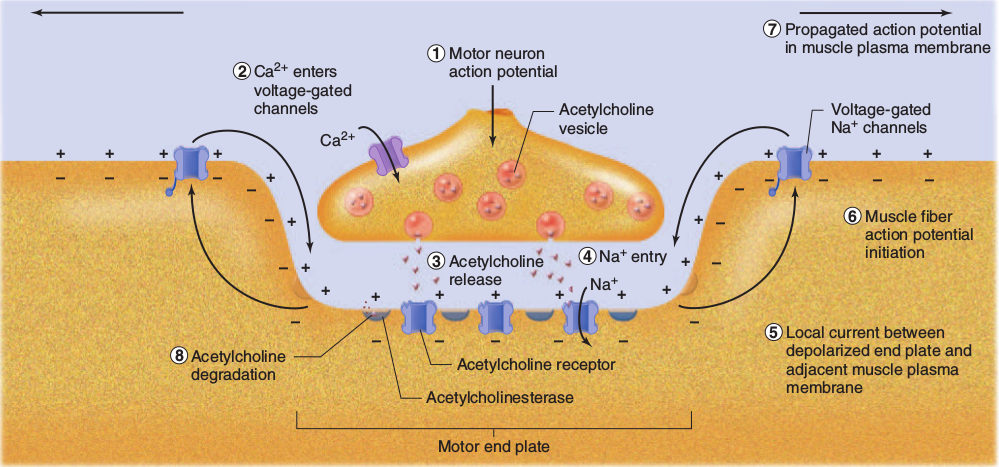
\includegraphics[width=0.95\textwidth]{Images/introduction/action_potential_generation.png}
\caption{Illustration of generation of action potential. Retrieved from \citep{Widmaier2014}.}
\label{fig:action_potential_generation}
\end{figure}
  
If the amount of acetylcoline is sufficient for the excitation, depolarization/repolarization wave, that is, action potential, propagates longitudinally from the neuromuscular junction towards the ends of the muscle fiber causing contraction \citep{Henneberg1999}. Speed of action potential propagation is called \emph{conduction velocity} and typically ranges around 4 m/s.

Detailed analysis of muscle physiology can be found elsewhere \citep{Squire1986, Widmaier2014}.






\section{Muscle fatigue}

Muscle fatigue is a continuous process that starts at the moment when muscle unit activates. If muscle keeps contracting long enough, eventually it will stop contracting because of electro-physiological inability to maintain the contraction. This moment is called the failure point \citep{DeLuca1984}. The failure point depends on many different factors physiological characteristics, but also on the number of muscle fibers and proportion of Type I/Type II muscle fibers. Muscles with higher proportion of Type I fibers do not fatigue easily and recover sooner than type II fibers. However, type II fibers are able to generate higher forces \citep{Kupa1995}.

Factors causing fatigue can be found in the muscle itself, in which case we talk about \emph{peripheral fatigue}, but can also 

Muscle during contraction develops muscle fatigue. It is characterized by decrease of conduction velocity \textbf{Wdimaier}. Although muscle fatigue begins to develop at the beginning of contractions, it is a challenge to grade it during contraction. What   

\begin{figure}[ht]
\centering
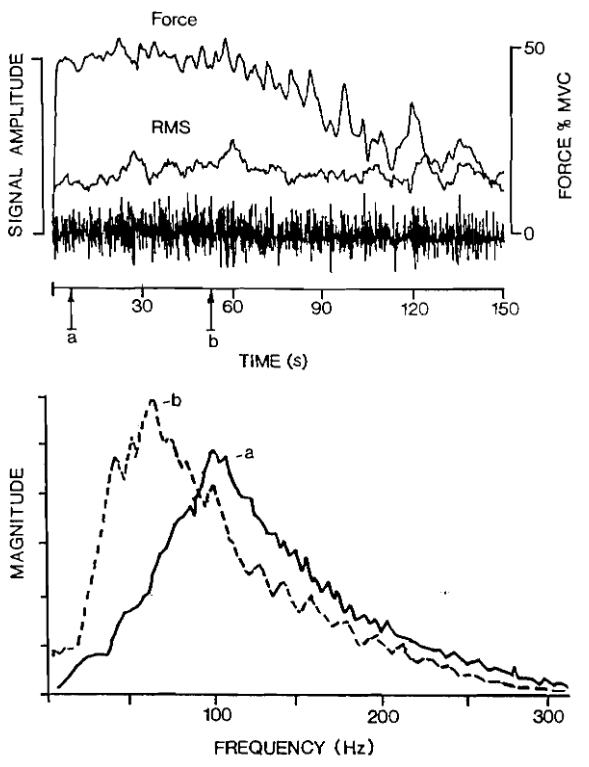
\includegraphics[width=0.45\textwidth]{Images/introduction/fatigue.png}
\caption{Illustration of force and EMG signal recorded during fatiguing exercise (top), and frequency spectra of corresponding EMG signal (bottom) recorded at the beginning of the exercise (a), and at the end of the exercise (b). Retrieved from \citep{DeLuca1984}.}
\label{fig:fatigue}
\end{figure}

\section{Surface electromyography}

Muscle unit action potentnial (MUAP) is the combination of action potentials generated by the single motor unit.
Myoelectric signal is a superposition of electrical activity (propagating action potentials) produced by the muscle fibers while contracting. 

EMG signals could be recorded either non-invasively (surface EMG, sEMG) or invasively with needle and wire electrodes (intramuscular EMG, iEMG) \citep{Marateb1999}. Although iEMG signal is usually with higher quality (in terms of signal-to-noise ratio), it was shown that both approaches provide a similar identification rate of upper-arm motor task \citep{Hargrove2007}.

Surface electromyographic signal (sEMG) is the sum of the electrical activity of the muscle fibers recorded on the surface of the skin. Since muscle fibers are activated by the impulse train of the innervating motor neurons, i.e. neural drive to the muscle, sEMG is the convolution of motor neuron spike trains by the motor unit action potential recorded on the electrodes \citep{Farina2010, Farina2014}:
\begin{equation}
sEMG(t) = \sum_{i=1}^{M} \sum_{j=-\infty}^{+\infty} MUAP_i(t)\,\, \delta(t-t_{i,j})
\end{equation}
, where $M$ is the number of active motor units, $MUAP_i(t)$ is the action potential waveform of the $i^{th}$ motor unit recorded by the electrodes, and $t_{i,j}$ is the time of the discharge of the $i^{th}$ motor neuron. This model assumes there is no interference and that neuromuscular junction never fails, which is not the case. In the equation, $MUAP_i(t)$ is related to the electrophysiological state of the muscle fiber membranes and conduction properties of the tissue through which the potential propagates, whereas neural information is contained in motor neuron spike trains $\delta(t-t_{i,j})$ \citep{Farina2014b}. It is important to notice that following this model, sEMG reflects all information that is present in motor neuron. Therefore, it is more appropriate to extract motor control information carried by motor neurons using sEMG, than directly by invasive measurement of electrical potential of the motor neuron. The advantage of the sEMG is that multiple fibers are activated simultanously, generating bioelectrical signal with relatively high SNR, which can be measured on the surface of the skin. In this context, sEMG can be considered as the amplified neural signal, whereas muscle can be considered as biological amplifier of nerve activity \citep{Farina2014}. Origin of sEMG signal can be seen in figure \ref{fig:EMG_origin}.
\begin{figure}[ht]
\centering
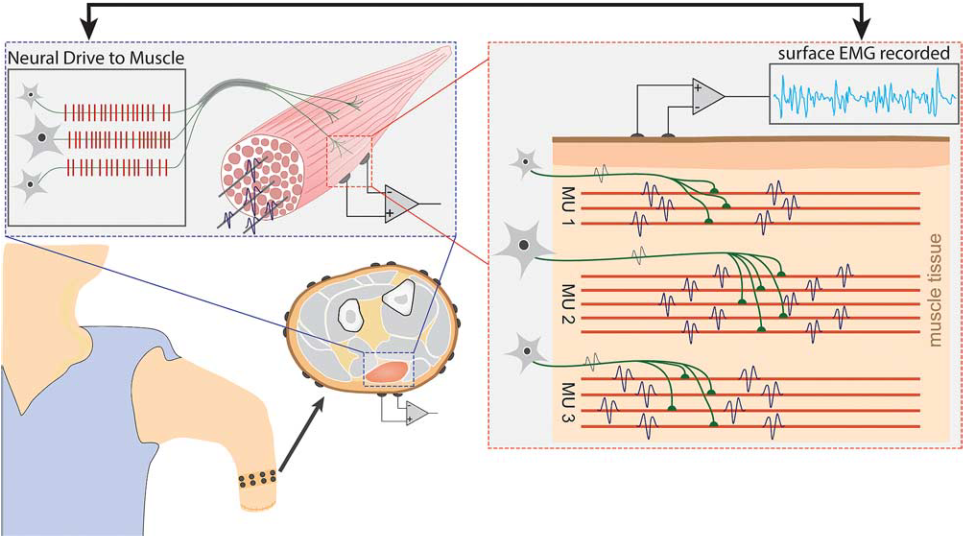
\includegraphics[width=0.75\textwidth]{Images/introduction/EMG_origin.png}
\caption{Origin of sEMG signal. SEMG signal is a sum of each motor unit action potential recorded on the electrodes convoluted by belonging motor neuron spike train. Retrieved from \citep{Farina2014}.}
\label{fig:EMG_origin}
\end{figure}



Depending on number of electrodes used for the recording. the following classification exists: monopolar, bipolar, linear electrode array, and high-density EMG (see Figure \ref{fig:electrode_types})

\begin{figure}[ht]
\centering
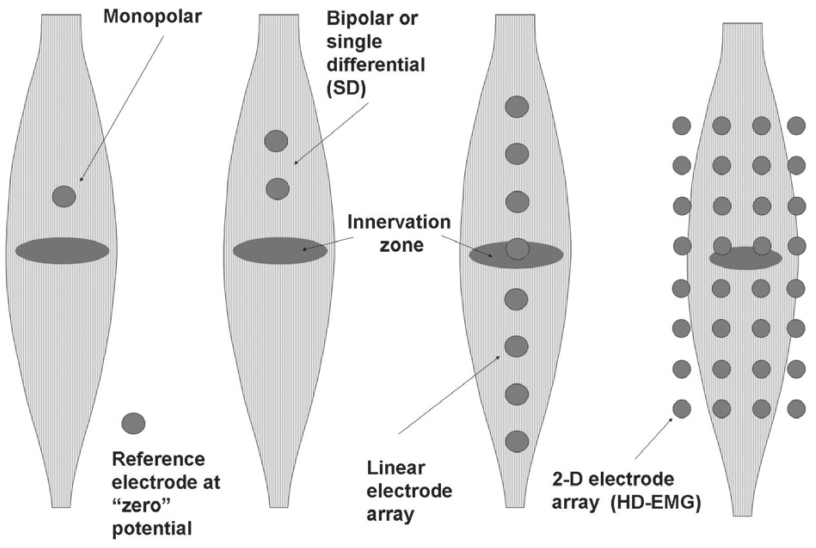
\includegraphics[width=0.55\textwidth]{Images/introduction/electrode_types.png}
\caption{Four types of recording surface EMG signal: monopolar, bipolar, linear electrode array, HD-EMG. Figure was modified from \citep{Merletti2010}}
\label{fig:electrode_types}
\end{figure}


Technological advancement of EMG acquisition systems enables use of high-density electromyography (HD-EMG) \citep{Zwarts2004}. Using an array of closely spaced electrodes organized in a quadrature grid, a wide muscle area is recorded. This technology is the only one that allows insights into spatial distribution of motor units in a muscle. By observing the amplitude or intensity of signals recorded in different channels, it is possible to analyze how different muscle regions activate depending on joint position \citep{Vieira2010}, contraction level \citep{Holtermann2005}, and duration of movement and fatigue \citep{Tucker2009, Staudenmann2014}. 

In addition, activation of individual motor units, i.e. individual motor neuron spike train, can be extracted from the HD-EMG recordings using Blind Source Separation methods \citep{Holobar2007, Holobar2010}, which can be a valuable information in force estimation because motor unit recruitment and firing frequency depend primarily on force level \citep{Merletti-book}. Several authors have used this approach instead of the traditional one based on intramuscular (invasive) EMG. One of the obvious advantages of this method is that is safe and not painful, although it has not been implemented in clinical practice yet. Using this technique, authors in \citep{Holobar2010} were able to extract 6 to 7 motor units starting from contractions at 5\% MVC and up to 20\% MVC with associated discharge rates between 10 pps and 12 pps. However, one of the current limitations is that the intensity of isometric contraction must remain constant during the measurement.

Similar algorithms can also be used to separate EMG activity of adjacent muscles \citep{Farina2004, Holobar2014}. This method can be a powerful tool in task identification \citep{Naik2007}, because it could minimize crosstalk effect from nearby muscles. Consequently, extracted features would characterize only the target muscles.
However, HD-EMG can be corrupted by low quality channels, which are a common issue in measurements due to well-known artifacts, such as: electrode displacement, bad electrical contact between skin and the electrode, movement of cables, electromagnetic interference, etc. \citep{Clancy2002b}. Affected channels differentiate themselves in amplitude and spectral content, which makes them outliers that compromise classification. To cope with this problem, authors in \citep{Rojas-Martinez2012} developed an expert system for detection, removal and interpolation of HD-EMG channels corrupted by artifacts.



\section{Task identification}


The central nervous system (CNS) is responsible for processing information received from all parts of the body. The two main organs of the CNS are the brain and the spinal cord and are entirely composed of two kinds of specialized cells: neurons and glia. The brain is the most complex part of the human body and exerts a centralized control over the other organs. Neurons, the basic working units of the brain, are designed to transmit information within the brain to other nerve cells and to communicate with muscles and gland cells. The complex architecture of the brain is built on the extensive number of interconnected neurons sharing information through specialized connections called synapses. This connection allows  neurons to communicate through an electrical or chemical signals, producing ionic currents that generate electric and magnetic fields. 

The CNS is organized in multiple levels, from simple connections between cells to coordinated cell populations, building a complex architecture of interconnected brain regions. The neural processes at this last level are produced by the dynamic coordination of smaller elements. In the cerebral cortex, all this brain activity is summed and its electric and magnetic fields can be measured on the scalp surface. 


In most of the commercial prosthesis \citep{Parker1986}, sEMG of two muscles is recorded. In this simple scheme a single Degree-of-Freedom (DOF) can be controlled: the EMG amplitude of one muscle controls the output of one direction, whereas the EMG amplitude of the other muscle controls the other direction. If prosthesis needs to operate in multiple DOFs, a subject needs to switch between currently active DOF either by co-contraction or by pressing a switch button. In any case, the method is not intuitive nor efficient for the user \citep{Farina2014}.

Pattern recognition is an alternative to conventional control algorithms. The prerequisite of using pattern recognition for task identification is the presence of a pattern that can be extracted from the EMG signal. Major advancement over conventional conventional switching myocontrol is the possibility of.

Pattern recognition approach does not support proportional and simultaneous control for multiple motor tasks. Therefore, tasks need to be performed sequentially. This type of control prevents the user from achieving a fluid movement, but also demands planning of movement execution. Although pattern recognition improves the possibility, it has serious limitations. 

This implies sequential control which prevents the subject from doing fluent, e.g. Davidge et al. designed a system where movements that combine DoFs are labeled as unique classes in LDA problem, whereas Young et al. \citep{Young2013} propose system of parallel LDA classifiers that use conditional probabilities to separate between combination of tasks.

Proportional review \citep{Fougner2012}
Force can be estimated based on the EMG : \citep{Staudenmann2010}

In pattern recognition, there is still a large gap between industry and practice \citep{Jiang2012}.

On the other hand, one of the disadvantages of pattern recognition is the fact that in spite of the high accuracy, an error could lead to the completely unwanted task. Also, although identification rate is usually very high during the stationary task, errors often occur during transition between tasks. This problems can be partially prevented by employing the e.g. majority voting principle \citep{Englehart2003} (300ms, LDA), or decision-based velocity ramp that attenuates the velocity of a movement after the change of a task \citep{Simon2011}. 

Challenges in pattern recognition are electrode shift \citep{Hargrove2008, Young2011}, change in arm posture \citep{Fougner2011}, slow time dependent changes \citep{Farina2014} such as fatigue \citep{Tkach2010}, and change in electrode-skin impedance \citep{Clancy2002a}.


Future works: dynamic system, hybrid system

\subsection{Pattern recognition}

Given the one to one relationship between the neural commands and the activation of motor units in the muscles, surface electromyography (sEMG) has been used for more than a half of century as a noninvasive and natural way of extracting motor control information for identification of motion intention. Such information is used in numerous applications in rehabilitation engineering, e.g., prosthetics \citep{Li2010, Young2013, Stango2015}, exoskeletons \citep{VacaBenitez2013} and rehabilitation robots \citep{Dipietro2005, Marchal-Crespo2009}.
Ideally, an identification system should fulfill the following criteria \citep{Farina2014}:
\begin{itemize}
\item Intuitive control: simultaneous and proportional
\item Insensitive to changes in electrode - skin impedance,
\item Adaptive to changes during the use, i.e. fatigue, electrode-skin impedance change due to sweating and drying of conductive gel
\item Insensitive to precise position of electrodes
\item Fast and easy training procedure (ideally none)
\item Real time identification, i.e. time delay less than 300 ms \citep{Oskoei2007}
\item Low computation complexity which enables implementation in battery-powered device
\end{itemize}

Pattern recognition – based control strategy enables proportional usage of multiple DoFs without switching between states, which makes it more intuitive. According to Oskoei et al. \citep{Oskoei2007}, this strategy includes four main modules:
\begin{description}
\item[Data segmentation:] Comprises various techniques and methods that are used to handle data before feature extraction
\item[Feature extraction:] This module computes and presents preselected features for a classifier. Features, instead of raw signals, are fed into a classifier to improve classification efficiency. Selection or extraction features is one of the most critical stages in myoelectric control design.
\item[Classification:] A classification module recognizes signal patterns, and classifies them into predefined categories. Due to the complexity of biological signals, and the influence of physiological and physical conditions, the classifier should be adequately robust.
\item[Controller:] Generates output commands based on signal patterns and control schemes. Post-processing methods, such as majority voting, which are often applied after classification to eliminate destructive jumps and make a smooth output, are included in this module too.
\end{description}

The main drawback of this method is that only one movement can be activated at the time. Any task that requires more than one DoF must be performed sequentially. However, several authors recently proposed solutions which enable simultaneous control \citep{Young2013, Kamavuako2013, Baker2010}. A variety of classifiers (e.g. hidden Markov model, support vector machine, artificial neural network, fuzzy logic and linear discriminant analysis) \citep{Oskoei2007} has been used in myocontrol research. Nevertheless, multiple authors agree that the identification does not significantly depend on the classifier type \citep{Hargrove2007, Zhang2012, Hakonen2015}. Therefore, simple and easy to train classifiers like linear discriminant analysis (LDA) are preferred \citep{Li2010, Englehart1999, Tkach2010, Li2014, Hakonen2015}. On the other hand, finding an appropriate set of features is challenging \citep{Englehart1999, Tkach2010, Liu2013}. In literature, a lot of feature types were considered: 

\begin{description}
\item[Time domain features:] mean absolute value \citep{Hudgins1993}, integrated EMG \citep{Park1998}, variance \citep{Park1998, Zardoshti1995}, root mean square \citep{Farrell2008}, waveform length \citep{Hudgins1993}, zero crossing \citep{Hudgins1993}, log detector \citep{Tkach2010}, Wilson amplitude \citep{Zardoshti1995}, slope sign change \citep{Hudgins1993}, autoregressive coefficients \citep{Hargrove2007}, Cepstral coefficients \citep{Park1998}, mean absolute value slope \citep{Phinyomark2012}, histogram of EMG \citep{Phinyomark2012, Zardoshti1995}
\item[Frequency domain features:] mean frequency \citep{Phinyomark2012b}, median frequency \citep{Phinyomark2012b}, modified mean frequency \citep{Phinyomark2009}
\item[Time-frequency domain features:] short time Fourier transform \citep{Englehart2003b, Englehart2001}, continuous wavelet transform \citep{Englehart2003b, Englehart2001}, discrete wavelet transform \citep{Englehart2003b}, stationary wavelet transform \citep{Englehart2003b}, wavelet packet transform \citep{Englehart2003b, Englehart2001, Chu2006}
\item[Spatial domain features:] Experimental periodogram \citep{Stango2015}, center of gravity \citep{Rojas-Martinez2012, Rojas-Martinez2013}
\end{description}

Time domain features are commonly used \citep{Hakonen2015} because they achieve high identification accuracy and are computationally efficient.

However, Zwartz et al. \citep{Zwarts2003} pointed out that single channel EMG disregards important spatial aspects of MUAP propagation, which are essential for the force-generating capacity of the muscle, and, if not well addressed, can lead to incorrect conclusions. Moreover, since muscles do not activate homogeneously, single bipolar channel EMG has some serious drawbacks, which can be overcome by using 2D electrode arrays: high density EMG (HD-EMG). 

In HD-EMG measurements, multiple EMG channels are recorded using an array of closely spaced electrodes placed over the wide area of the muscle. This type of recording is more reliable because it can record activations in different parts of the muscle and increase redundancy. Commonly, authors in literature report identification based on HD-EMG and time domain features or autoregressive features calculated for each channel \citep{Hakonen2015}. Zhang et al. \citep{Zhang2012}, for example, used combination of these features with dimensionality reduction to identify 20 wrist and hand movements, and Muceli and Farina \citep{Muceli2012} performed estimation of hand kinematics during more than 20 movements using EMG envelopes as features with reduced dimensionality of channels.

But HD-EMG recordings also allow calculation of two-dimensional activation maps where intensity of each pixel represents the intensity of a corresponding EMG channel (see figure \ref{fig:HD-EMG}). Consequently, information on spatial distribution of EMG intensity over the muscle is provided. Recent studies show that changes in spatial activation pattern are related to duration of movement and fatigue \citep{Tucker2009, Staudenmann2014}, position of joint \citep{Vieira2010} and the level of contraction \citep{Holtermann2005}. Since spatial distribution contains a lot of information on the muscle, it is acknowledged as a valuable feature in identification of motion intention \citep{Stango2015, Hakonen2015, Rojas-Martinez2013}. For example, Stango et al. \citep{Stango2015} used spatial characteristics of HD-EMG recording of the forearm muscles to identify 8 hand and wrist tasks (4 degrees of freedom). They fed support vector machine classifier with a statistical measure of spatial correlation, i.e. variogram and achieved high identification results (95\% accuracy). Furthermore, they proved that proposed spatial features are robust to electrode shift.
\begin{figure}[ht]
\centering
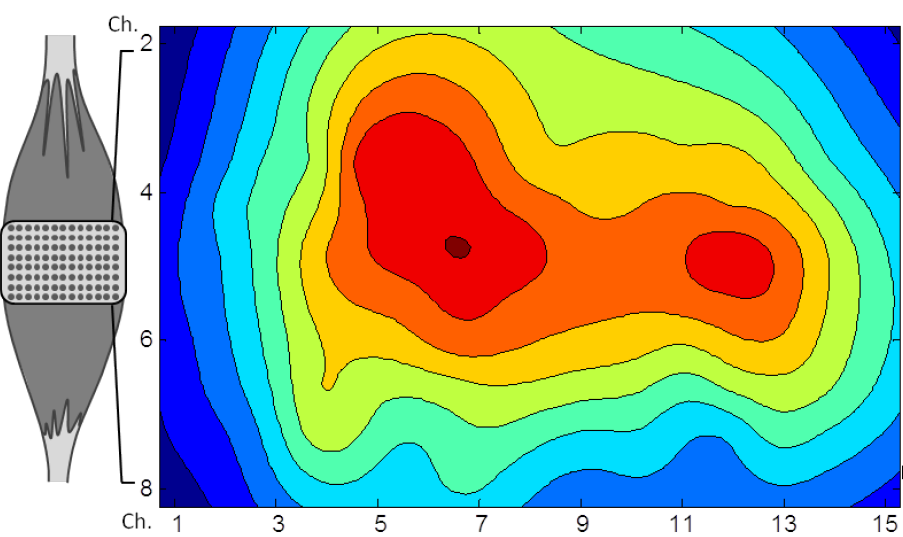
\includegraphics[width=0.95\textwidth]{Images/introduction/HD-EMG.png}
\caption{The figure represents the HD-EMG activation map recorded on the biceps brachii muscle during flexion. Distinct activation of the two heads can be noticed in the map. Modified from Monica}
\label{fig:HD-EMG}
\end{figure}

Most of pattern recognition identification methods are subject-specific. They usually achieve very high identification results, but require time consuming training procedure for every patient individually. This could be avoided by building a single identifier for a group of patients, i.e. group-specific identifier. However, inter-subject variability is a big concern in design of a group-specific pattern recognition-based identifier. Individuals differ from each other in a lot of physiological parameters, e.g., conductivity of subcuntaneous tissue, and limb dimension. Nevertheless, by comparing HD-EMG activation maps between normal subjects it has been shown that inter-subject activation patterns exists for different tasks and levels of contraction \citep{Rojas-Martinez2012}.

In \citep{Rojas-Martinez2013} authors demonstrate that by using intensity and spatial features extracted from activation maps it is possible to construct an inter-subject identification method based on LDA classifier not only for different tasks, but also for different effort levels. Authors reported that in healthy subjects identification performance improves by adding spatial features in the identification, which proves that spatial distribution is less sensitive to inter-subject variability. They achieved sensitivity higher than 75\% for identification of four upper-limb tasks at three different effort levels and more than 90\% sensitivity when identifying only four tasks and no effort level. Also, they report higher classification results when using classification in two steps (in first step task is classified, and in the second step level of effort), rather than a single step classification.



\subsection{Application to patients with neuromuscular impairment}
According to World Health Organization, each year there are 500 000 spinal cord injuries [56] and 15 million strokes (of which 5 million result with death and 5 million with permanent disability) [57] every year. Furthermore, number of people who are older than 60 years will increase to 22\% of the world population by 2050 and will count 2 billion people [58]. Unfortunately, in affected patients motor control can be impaired as a result of damaged nerves and they often suffer from uncoordinated movements, lack of force, and spasticity. During recovery process, rehabilitation robots that stimulate neuroplasticity are commonly used \citep{VacaBenitez2013, Dipietro2005, Marchal-Crespo2009}. 

Patients can still have uncoordinated movements, and lack of force, or, in more difficult cases, they can weakly activate their muscles, but cannot perform the movement. If their motion intention could be extracted in real time, it would allow them to control assistive devices and maximize the benefits of robotic-aided therapies where it has been proved that the active participation improves the medical condition of the patient \citep{Hogan2006}.

It is already shown that intensity-related and task-specific activation patterns exist in patients with neurological disorders and that motion intention can be extracted from EMG. In other words, movement that patient is trying to perform can be predicted using the recorded myoelectric activity. Liu and Zhou \citep{Liu2013} were able to successfully perform identification of tasks using time domain and autoregressive model features in patients with incomplete spinal cord injury, whereas Zhang and Zhou \citep{Zhang2012} identified tasks in patients with stroke using a similar feature set.




Physical injury to the brain, spinal cord, or nerves, is usually the cause of neurological disorders.
Stroke is a serious life-threatening condition that occurs when the blood supply to the brain is interrupted, resulting in severe disability among survivors. Brain damage due to stroke can affect important areas that control everything we do, including how we move different parts of our body.

In disabling neurological disorders, treatment and rehabilitation should start as soon as possible after the diagnosis. This situation is critical in stroke patients where rehabilitation usually begins two days after the stroke has occurred. Early intervention can improve bodily functions and even achieve remarkable recoveries, and should be continued as necessary after release from the hospital to become as independent as possible. Rehabilitation can help regain control of weak limbs, or learn new ways of using them again, that is, to relearn skills that are lost when part of the brain is damaged, mainly associated with motor capabilities.

Human-machine interfaces cannot only translate brain signals to control targets, but also can combine with a muscle-based output. This hybrid approach is composed of multimodal data from the brain (EEG) and from the muscles (EMG), especially important for patients with residual muscular activity. Additionally, corticomuscular coherence assessed through both EEG and EMG signals is a promising measure to evaluate the motor recovery of stroke patients. This Project is on monitoring the patient's progress during the rehabilitation program, and biomarkers composed of EMG and EEG information will be very interesting. For example, Transcranial Magnetic Stimulation (TMS) has been used to probe corticospinal physiology and to map the primary motor cortex (M1) representations of upper limb muscles following stroke.

its application to pattern recognition to provide a control signal to interfaces like prostheses or rehabilitation robots, particularly for stroke or other neuromuscular disorders

Common manifestations of upper extremity motor impairment include muscle weakness or contracture, changes in muscle tone, joint laxity, and impaired motor control. These impairments induce disabilities in common activities such as reaching, picking up objects, and holding onto objects.

The aim of this research line is to analyze biological signals of patients undergoing stroke rehabilitation and extract measures that reflect the current degree of recovery and neuromuscular ability, and to define and evaluate expert-based quantitative indices for
predicting the final clinical outcome of the standard 6-month rehabilitation. This latter aim would be very useful for the physicians leading the therapy and would save a lot of time and resources. For example, if a patient is not able to achieve true recovery of the affected motor function, he could start with an alternative treatment immediately and learn a compensatory motor task, improving its quality of life faster. According to rehabilitation professionals, these particular cases are very difficult to identify early on, and it takes months before realizing that a different approach is needed. On the other hand, if the measure indicates a good recovery potential, it would be possible to tailor a patient-oriented rehabilitation program that would maximize its effect.

Neural data can be inferred from HD-EMG signal using HD-EMG decomposition to spike train of individual motor units (Holobar et al., 2014, Negro et al., 2016). This technique enables measuring of valuable information about muscle unit recruitment: muscle fiber conduction velocity, location of the innervation zones, estimation of muscle fatigue, and estimation of number, type and the spatial distribution of muscle fibers (Marateb et al., 2016). Other potential measures that can be found in the literature are the clustering index (Zhang et al., 2017), measures based on textural and spatial analysis of HD-EMG activation maps (Rasool et al., 2017), the coherence between muscle units (Dai et al., 2017), or measures based on muscle synergies (Li et al., 2016). The advantages of the HD-EMG lie in the large amount of recorded information, which enables minimizing the effect of electrodes shift and allows choosing an appropriate subset of channels for further analysis. Features will be designed by optimizing its robustness to electrode shift and minimizing the number of electrodes, which is an important issue in HD-EMG analysis (Pan et al., 2015), but also in EEG analysis and BCI systems
(Alotaiby et al., 2015, Tam et al., 2011).

Stroke patients often do not have the ability to achieve a specific task, even though they maintain correct neuromuscular activation, due to spasticity or insufficient contraction (i.e. insufficient force) (Liu et al., 2016). However, it can be possible to observe both, the neural
and muscular response (potentials) to motor intention in absence of joint movement. Lack of movement can be a misleading factor in clinical assessment and the design of the rehabilitation program. Accurate task identification would provide clinicians with the patient’s real capabilities and potential.




\subsection {Doctoral thesis overview}

This doctoral thesis is presented as the compendium of three publications. 

The Doctoral Thesis is organized by chapters as follows:

\begin{itemize}
\item \textbf{Chapter 2: Problem statement}\\
	This chapter states the problem and provides the objectives of Doctoral Thesis.
	
\item \textbf{Chapter 3: Spatial distribution of HD-EMG improves identification of task and force in patients with incomplete spinal cord injury}\\
	This chapter represents the first publication of the compendium of publications. Using spatial distribution of myoelectric intensity task identification was performed on patients with incomplete spinal cord injury. This work proves the positive contribution of spatial features in pattern recognition technique of identification of motor tasks. Not only that the identification rate increases, but the features show resilience to slow time dependent changes in the myoelectric signal, such as fatigue and drying of electrolytic gel
	
\item \textbf{Chapter 4: Prediction of isometric motor tasks and effort levels based on high-density EMG in patients with incomplete spinal cord injury}\\
	In this publication, the similarity of intensity and spatial distribution of intensity was investigated between patients with incomplete spinal cord injury. The results show that the repeatable pattern exists between different patients and, moreover, for the patients with similar level of injury this patterns are more similar.

\item \textbf{Chapter 5: A Novel Spatial Feature for the Identification of Motor Tasks Using High-Density Electromyography}\\
	This chapter summarizes the  third publication of the compendium. The novel feature was designed for task identification. It is based on probability density function of HD-EMG activation maps. Classifier based on this new feature show higher identification rate, as well as fidelity to fatigue.

\item \textbf{Conclusions}\\
	In the last chapter, the conclusions and main contributions of the Thesis are provided. Also, the guidelines for the future work are stated, as well as list of publications derived from the Thesis.

\end{itemize}





\

